\documentclass[12pt,twoside]{article}

\newcommand{\reporttitle}{Machine Learning}
\newcommand{\reportauthor}{Dimitrogiannis Kontogouris, Michael Tarasiou}
\newcommand{\reporttype}{CBC: Neural Networks}
\newcommand{\cid}{00650270}
\usepackage{amsmath}
\usepackage{listings}
\usepackage{lscape}
\usepackage{float}

% include files that load packages and define macros
%%%%%%%%%%%%%%%%%%%%%%%%%%%%%%%%%%%%%%%%%
% University Assignment Title Page 
% LaTeX Template
% Version 1.0 (27/12/12)
%
% This template has been downloaded from:
% http://www.LaTeXTemplates.com
%
% Original author:
% WikiBooks (http://en.wikibooks.org/wiki/LaTeX/Title_Creation)
%
% License:
% CC BY-NC-SA 3.0 (http://creativecommons.org/licenses/by-nc-sa/3.0/)
% 
% Instructions for using this template:
% This title page is capable of being compiled as is. This is not useful for 
% including it in another document. To do this, you have two options: 
%
% 1) Copy/paste everything between \begin{document} and \end{document} 
% starting at \begin{titlepage} and paste this into another LaTeX file where you 
% want your title page.
% OR
% 2) Remove everything outside the \begin{titlepage} and \end{titlepage} and 
% move this file to the same directory as the LaTeX file you wish to add it to. 
% Then add \input{./title_page_1.tex} to your LaTeX file where you want your
% title page.
%
%----------------------------------------------------------------------------------------
%	PACKAGES AND OTHER DOCUMENT CONFIGURATIONS
%----------------------------------------------------------------------------------------
\usepackage{ifxetex}
\usepackage{textpos}
\usepackage{natbib}
\usepackage{kpfonts}
\usepackage[a4paper,hmargin=2.8cm,vmargin=2.0cm,includeheadfoot]{geometry}
\usepackage{ifxetex}
\usepackage{stackengine}
\usepackage{tabularx,longtable,multirow,subfigure,caption}%hangcaption
\usepackage{fncylab} %formatting of labels
\usepackage{fancyhdr}
\usepackage{color}
\usepackage[tight,ugly]{units}
\usepackage{url}
\usepackage{float}
\usepackage[english]{babel}
\usepackage{amsmath}
\usepackage{graphicx}
\usepackage[colorinlistoftodos]{todonotes}
\usepackage{dsfont}
\usepackage{epstopdf} % automatically replace .eps with .pdf in graphics
\usepackage{natbib}
\usepackage{backref}
\usepackage{array}
\usepackage{latexsym}
\usepackage{etoolbox}

\usepackage{enumerate} % for numbering with [a)] format 



\ifxetex
\usepackage{fontspec}
\setmainfont[Scale=.8]{OpenDyslexic-Regular}
\else
\usepackage[pdftex,pagebackref,hypertexnames=false,colorlinks]{hyperref} % provide links in pdf
\hypersetup{pdftitle={},
  pdfsubject={}, 
  pdfauthor={\reportauthor},
  pdfkeywords={}, 
  pdfstartview=FitH,
  pdfpagemode={UseOutlines},% None, FullScreen, UseOutlines
  bookmarksnumbered=true, bookmarksopen=true, colorlinks,
    citecolor=black,%
    filecolor=black,%
    linkcolor=black,%
    urlcolor=black}
\usepackage[all]{hypcap}
\fi

\usepackage{tcolorbox}

% various theorems
\usepackage{ntheorem}
\theoremstyle{break}
\newtheorem{lemma}{Lemma}
\newtheorem{theorem}{Theorem}
\newtheorem{remark}{Remark}
\newtheorem{definition}{Definition}
\newtheorem{proof}{Proof}

% example-environment
\newenvironment{example}[1][]
{ 
\vspace{4mm}
\noindent\makebox[\linewidth]{\rule{\hsize}{1.5pt}}
\textbf{Example #1}\\
}
{ 
\noindent\newline\makebox[\linewidth]{\rule{\hsize}{1.0pt}}
}



%\renewcommand{\rmdefault}{pplx} % Palatino
% \renewcommand{\rmdefault}{put} % Utopia

\ifxetex
\else
\renewcommand*{\rmdefault}{bch} % Charter
\renewcommand*{\ttdefault}{cmtt} % Computer Modern Typewriter
%\renewcommand*{\rmdefault}{phv} % Helvetica
%\renewcommand*{\rmdefault}{iwona} % Avant Garde
\fi

\setlength{\parindent}{0em}  % indentation of paragraph

\setlength{\headheight}{14.5pt}
\pagestyle{fancy}
\fancyfoot[ER,OL]{\thepage}%Page no. in the left on
                                %odd pages and on right on even pages
\fancyfoot[OC,EC]{\sffamily }
\renewcommand{\headrulewidth}{0.1pt}
\renewcommand{\footrulewidth}{0.1pt}
\captionsetup{margin=10pt,font=small,labelfont=bf}


%--- chapter heading

\def\@makechapterhead#1{%
  \vspace*{10\p@}%
  {\parindent \z@ \raggedright %\sffamily
        %{\Large \MakeUppercase{\@chapapp} \space \thechapter}
        %\\
        %\hrulefill
        %\par\nobreak
        %\vskip 10\p@
    \interlinepenalty\@M
    \Huge \bfseries 
    \thechapter \space\space #1\par\nobreak
    \vskip 30\p@
  }}

%---chapter heading for \chapter*  
\def\@makeschapterhead#1{%
  \vspace*{10\p@}%
  {\parindent \z@ \raggedright
    \sffamily
    \interlinepenalty\@M
    \Huge \bfseries  
    #1\par\nobreak
    \vskip 30\p@
  }}
  



% %%%%%%%%%%%%% boxit
\def\Beginboxit
   {\par
    \vbox\bgroup
	   \hrule
	   \hbox\bgroup
		  \vrule \kern1.2pt %
		  \vbox\bgroup\kern1.2pt
   }

\def\Endboxit{%
			      \kern1.2pt
		       \egroup
		  \kern1.2pt\vrule
		\egroup
	   \hrule
	 \egroup
   }	

\newenvironment{boxit}{\Beginboxit}{\Endboxit}
\newenvironment{boxit*}{\Beginboxit\hbox to\hsize{}}{\Endboxit}



\allowdisplaybreaks

\makeatletter
\newcounter{elimination@steps}
\newcolumntype{R}[1]{>{\raggedleft\arraybackslash$}p{#1}<{$}}
\def\elimination@num@rights{}
\def\elimination@num@variables{}
\def\elimination@col@width{}
\newenvironment{elimination}[4][0]
{
    \setcounter{elimination@steps}{0}
    \def\elimination@num@rights{#1}
    \def\elimination@num@variables{#2}
    \def\elimination@col@width{#3}
    \renewcommand{\arraystretch}{#4}
    \start@align\@ne\st@rredtrue\m@ne
}
{
    \endalign
    \ignorespacesafterend
}
\newcommand{\eliminationstep}[2]
{
    \ifnum\value{elimination@steps}>0\leadsto\quad\fi
    \left[
        \ifnum\elimination@num@rights>0
            \begin{array}
            {@{}*{\elimination@num@variables}{R{\elimination@col@width}}
            |@{}*{\elimination@num@rights}{R{\elimination@col@width}}}
        \else
            \begin{array}
            {@{}*{\elimination@num@variables}{R{\elimination@col@width}}}
        \fi
            #1
        \end{array}
    \right]
    & 
    \begin{array}{l}
        #2
    \end{array}
    &%                                    moved second & here
    \addtocounter{elimination@steps}{1}
}
\makeatother

%% Fast macro for column vectors
\makeatletter  
\def\colvec#1{\expandafter\colvec@i#1,,,,,,,,,\@nil}
\def\colvec@i#1,#2,#3,#4,#5,#6,#7,#8,#9\@nil{% 
  \ifx$#2$ \begin{bmatrix}#1\end{bmatrix} \else
    \ifx$#3$ \begin{bmatrix}#1\\#2\end{bmatrix} \else
      \ifx$#4$ \begin{bmatrix}#1\\#2\\#3\end{bmatrix}\else
        \ifx$#5$ \begin{bmatrix}#1\\#2\\#3\\#4\end{bmatrix}\else
          \ifx$#6$ \begin{bmatrix}#1\\#2\\#3\\#4\\#5\end{bmatrix}\else
            \ifx$#7$ \begin{bmatrix}#1\\#2\\#3\\#4\\#5\\#6\end{bmatrix}\else
              \ifx$#8$ \begin{bmatrix}#1\\#2\\#3\\#4\\#5\\#6\\#7\end{bmatrix}\else
                 \PackageError{Column Vector}{The vector you tried to write is too big, use bmatrix instead}{Try using the bmatrix environment}
              \fi
            \fi
          \fi
        \fi
      \fi
    \fi
  \fi 
}  
\makeatother

\robustify{\colvec}

%%% Local Variables: 
%%% mode: latex
%%% TeX-master: "notes"
%%% End: 
 % various packages needed for maths etc.
% quick way of adding a figure
\newcommand{\fig}[3]{
 \begin{center}
 \scalebox{#3}{\includegraphics[#2]{#1}}
 \end{center}
}

%\newcommand*{\point}[1]{\vec{\mkern0mu#1}}
\newcommand{\ci}[0]{\perp\!\!\!\!\!\perp} % conditional independence
\newcommand{\point}[1]{{#1}} % points 
\renewcommand{\vec}[1]{{\boldsymbol{{#1}}}} % vector
\newcommand{\mat}[1]{{\boldsymbol{{#1}}}} % matrix
\newcommand{\R}[0]{\mathds{R}} % real numbers
\newcommand{\Z}[0]{\mathds{Z}} % integers
\newcommand{\N}[0]{\mathds{N}} % natural numbers
\newcommand{\nat}[0]{\mathds{N}} % natural numbers
\newcommand{\Q}[0]{\mathds{Q}} % rational numbers
\ifxetex
\newcommand{\C}[0]{\mathds{C}} % complex numbers
\else
\newcommand{\C}[0]{\mathds{C}} % complex numbers
\fi
\newcommand{\tr}[0]{\text{tr}} % trace
\renewcommand{\d}[0]{\mathrm{d}} % total derivative
\newcommand{\inv}{^{-1}} % inverse
\newcommand{\id}{\mathrm{id}} % identity mapping
\renewcommand{\dim}{\mathrm{dim}} % dimension
\newcommand{\rank}[0]{\mathrm{rk}} % rank
\newcommand{\determ}[1]{\mathrm{det}(#1)} % determinant
\newcommand{\scp}[2]{\langle #1 , #2 \rangle}
\newcommand{\kernel}[0]{\mathrm{ker}} % kernel/nullspace
\newcommand{\img}[0]{\mathrm{Im}} % image
\newcommand{\idx}[1]{{(#1)}}
\DeclareMathOperator*{\diag}{diag}
\newcommand{\E}{\mathds{E}} % expectation
\newcommand{\var}{\mathds{V}} % variance
\newcommand{\gauss}[2]{\mathcal{N}\big(#1,\,#2\big)} % gaussian distribution N(.,.)
\newcommand{\gaussx}[3]{\mathcal{N}\big(#1\,|\,#2,\,#3\big)} % gaussian distribution N(.|.,.)
\newcommand{\gaussBig}[2]{\mathcal{N}\left(#1,\,#2\right)} % see above, but with brackets that adjust to the height of the arguments
\newcommand{\gaussxBig}[3]{\mathcal{N}\left(#1\,|\,#2,\,#3\right)} % see above, but with brackets that adjust to the height of the arguments
\DeclareMathOperator{\cov}{Cov} % covariance (matrix) 
\ifxetex
\renewcommand{\T}[0]{^\top} % transpose
\else
\newcommand{\T}[0]{^\top}
\fi
% matrix determinant
\newcommand{\matdet}[1]{
\left|
\begin{matrix}
#1
\end{matrix}
\right|
}



%%% various color definitions
\definecolor{darkgreen}{rgb}{0,0.6,0}

\newcommand{\blue}[1]{{\color{blue}#1}}
\newcommand{\red}[1]{{\color{red}#1}}
\newcommand{\green}[1]{{\color{darkgreen}#1}}
\newcommand{\orange}[1]{{\color{orange}#1}}
\newcommand{\magenta}[1]{{\color{magenta}#1}}
\newcommand{\cyan}[1]{{\color{cyan}#1}}


% redefine emph
\renewcommand{\emph}[1]{\blue{\bf{#1}}}

% place a colored box around a character
\gdef\colchar#1#2{%
  \tikz[baseline]{%
  \node[anchor=base,inner sep=2pt,outer sep=0pt,fill = #2!20] {#1};
    }%
}%
 % short-hand notation and macros


%%%%%%%%%%%%%%%%%%%%%%%%%%%%

\begin{document}
% front page
% Last modification: 2016-09-29 (Marc Deisenroth)
\begin{titlepage}

\newcommand{\HRule}{\rule{\linewidth}{0.5mm}} % Defines a new command for the horizontal lines, change thickness here


%----------------------------------------------------------------------------------------
%	LOGO SECTION
%----------------------------------------------------------------------------------------


\includegraphics[width = 4cm]{./figures/imperial}\\[0.5cm] 

\begin{center} % Center remainder of the page

%----------------------------------------------------------------------------------------
%	HEADING SECTIONS
%----------------------------------------------------------------------------------------
\textsc{\LARGE \reporttype}\\[1.5cm] 
\textsc{\Large Imperial College London}\\[0.5cm] 
\textsc{\large Department of Computing}\\[0.5cm] 
%----------------------------------------------------------------------------------------
%	TITLE SECTION
%----------------------------------------------------------------------------------------

\HRule \\[0.4cm]
{ \huge \bfseries \reporttitle}\\ % Title of your document
\HRule \\[1.5cm]
\end{center}
%----------------------------------------------------------------------------------------
%	AUTHOR SECTION
%----------------------------------------------------------------------------------------

%\begin{minipage}{0.4\hsize}
\begin{flushleft} \large
\textit{Author:}\\
\reportauthor~(CID: \cid) % Your name
\end{flushleft}
\vspace{2cm}
\makeatletter
Date: \@date 

\vfill % Fill the rest of the page with whitespace



\makeatother


\end{titlepage}



%%%%%%%%%%%%%%%%%%%%%%%%%%%% Main document


\section{Linear and Relu layers}
\subsection{Linear forward pass}

The linear forward function performs a linear transformation to the incoming data matrix $X \in \mathbb{R}^{N \times D}$, transforming it into a matrix $y \in \mathbb{R}^{N \times B}$ where $B$ is the number of neurons in the next layer of the network. Mathematically this is shown below:
\begin{align}
y = XW + b
\end{align}
The matrix b representing the biases of each neuron is a matrix of size $N \times B$. The rows are all the same, and in each column the bias of the corresponding neuron is stored.


\subsection{Linear backward pass}

For the backward pass, we are asked to return the derivatives of the loss function with respect to the weights and biases in the layer and the input X.
We have:
\begin{align}
dw = \frac{\partial L}{\partial w} = \frac{\partial L}{\partial y} \times \frac{\partial y}{\partial w}
\end{align}
\begin{align*}
\frac{\partial y}{\partial w} = \frac{\partial (XW + b)}{\partial w} = X
\end{align*}

We know $\frac{\partial L}{\partial y}$ since it is a function input (dout) and thus we can calculate $dw$:
\begin{align}
dw = \frac{\partial L}{\partial w} = \frac{\partial L}{\partial y} \times X = dout \times X
\end{align}
Similarly, the gradient with respect to the biases is:
\begin{align*}
db = \frac{\partial L}{\partial b} = \frac{\partial L}{\partial y} \times \frac{\partial y}{\partial b} = \frac{\partial L}{\partial y} \times 1 = \frac{\partial L}{\partial y} = dout
\end{align*}

Finally, the gradient with respect to the input X:
\begin{align}
dX = \frac{\partial L}{\partial X} = \frac{\partial L}{\partial y} \times \frac{\partial y}{\partial X} = \frac{\partial L}{\partial y} \times W = dout \times W
\end{align}

The dimensions of the gradients are the following:
\begin{itemize}
\item $dw \in \mathbb{R}^{D \times B}$
\item $db \in \mathbb{R}^{N \times B}$
\item $dX \in \mathbb{R}^{N \times D}$
\end{itemize}

\subsection{Relu forward pass}

The relu forward pass is simply defined as:
\begin{align}
y = max(0,X)
\end{align}
The output of the relu forward pass is the input X, if X is greater than 0, otherwise it is 0. The dimensions of matrices $y$ and $X$ are the same $N \times D$ for some $N$ and $D$.

\subsection{Relu backward pass}

The relu backward pass is simply 0 if X less than 0, otherwise it is equal to dout.

\section{Dropout}
Dropout is a method to prevent over-fitting in the neural network by "disabling" neurons in the layers of the network. Each neuron has a probability $p$ of being dropped.

\subsection{Dropout forward pass}
To perform the dropout forward pass, we create a matrix called $mask$ which is of the same shape as the input X, Each element of $mask$, is a random draw from a Bernoulli distribution, with $p$ probability of being $0$, and $1-p$ of being 1. The output of the layer is an element-wise multiplication of matrix $mask$ and the input $X$, and thus the result is a matrix equal to X, with some of its elements being equal to 0. In addition, the resulting matrix is scaled with a factor of $1/(1-p)$ since we are performing inverted dropout. This is only done during the training of the network.

\subsection{Dropout backward pass}

For the backward pass, we perform the same operation as for the forward pass in the opposite direction. We multiply the scaling factor, with the mask (the same as before!) and with the derivatives from previous layers which is an input in the functions. This is during the training phase. In the testing phase, the derivatives simply pass through, without a mask. 



\section{Softmax}

The output of the neural network produces a number for each of the classes we have in our classification problem. These numbers can be interpreted as un-normalized probabilities. Using a softmax function, we can normalize them, so that their sum adds up to 1.
Mathematically the softmax function is defined as:

\begin{align}
\sigma_j (y_i) = \frac{e^{y_i[j]}}{\sum_{k=1}^{D} e^{y_i[k]}}
\end{align}

where, D is the number of classes and $y_i \in \mathbb{R}^D$ is a vector with the outputs of the network for each class (of the $i_{th}$ sample). For numerical stability, we multiply (6) both the numerator and denominator by a constant K which improves stability without changing the results.



\subsection{Gradient of softmax}
For the combination of softmax and the negative log likelihood cost function we use, for a label $l \in \R^{D}$ we have the following:

\begin{align*}
L &= - \sum_j l_j \log \sigma_j
\end{align*}

\begin{align*}
\frac{\partial \sigma_j}{\partial y_j} &= \frac{\exp y_j \exp \sum_k y_k - (\exp y_j)^2}{(\sum_k \exp y_k)^2}= \sigma_j (1 - \sigma_j)\\
\\
\frac{\partial \sigma_j}{\partial y_i} &= \frac{-\exp y_j \exp y_i}{(\sum_k \exp y_k)^2}= -\sigma_j \sigma_i, \quad \forall i \neq j
\end{align*}

\begin{align*}
\frac{\partial L}{\partial y_i} &= -\frac{\partial l_i \sigma_i + \sum_{j \neq i}l_j \log \sigma_j}{\partial y_i}\\
&= - l_i \frac{1}{\sigma_i} (1-\sigma_i) \sigma_i + \sum_{j \neq i} l_j \frac{1}{\sigma_j} \sigma_j \sigma_i \\
&= \sigma_i \sum_j l_j - l_i = \sigma_i - l_i
\end{align*}\section{Fully connected Network}
\subsection{Architecture}
\subsection{L2-regularization}

\subsection{Overfitting}
For the overfitting task we selected the top 50 images and label from CIFAR10 and used just those to fit a model. Since the objective was to fit the training data as good as possible with no consideration of generalization capabilities of our network we had the following strategy:
\begin{itemize}
\item use a network with many nodes in the hidden layers. We selected a network with two hidden layers with 1024 and 512 nodes respectively
\item we did not apply any type of regularization as this would penalize the complexity of the model
\end{itemize}

The selected model achieves $100\%$ accuracy over the training set at the sixth epoch as can be shown in Fig.\ref{fig:overfit} below.
\\

To get $50\%$ accuracy over the validation set, we selected a network with two hidden layers, 512 and 256 nodes per respective layer. We didn't use dropout, but we did use a $0.2$ L2 regularization multiplier. The model achieved $>50\%$ over the validation set after 4 epochs as can be seen in Fig.\ref{fig:cifar_2layer} below. 

\begin{figure}[H]
\centering % this centers the figure
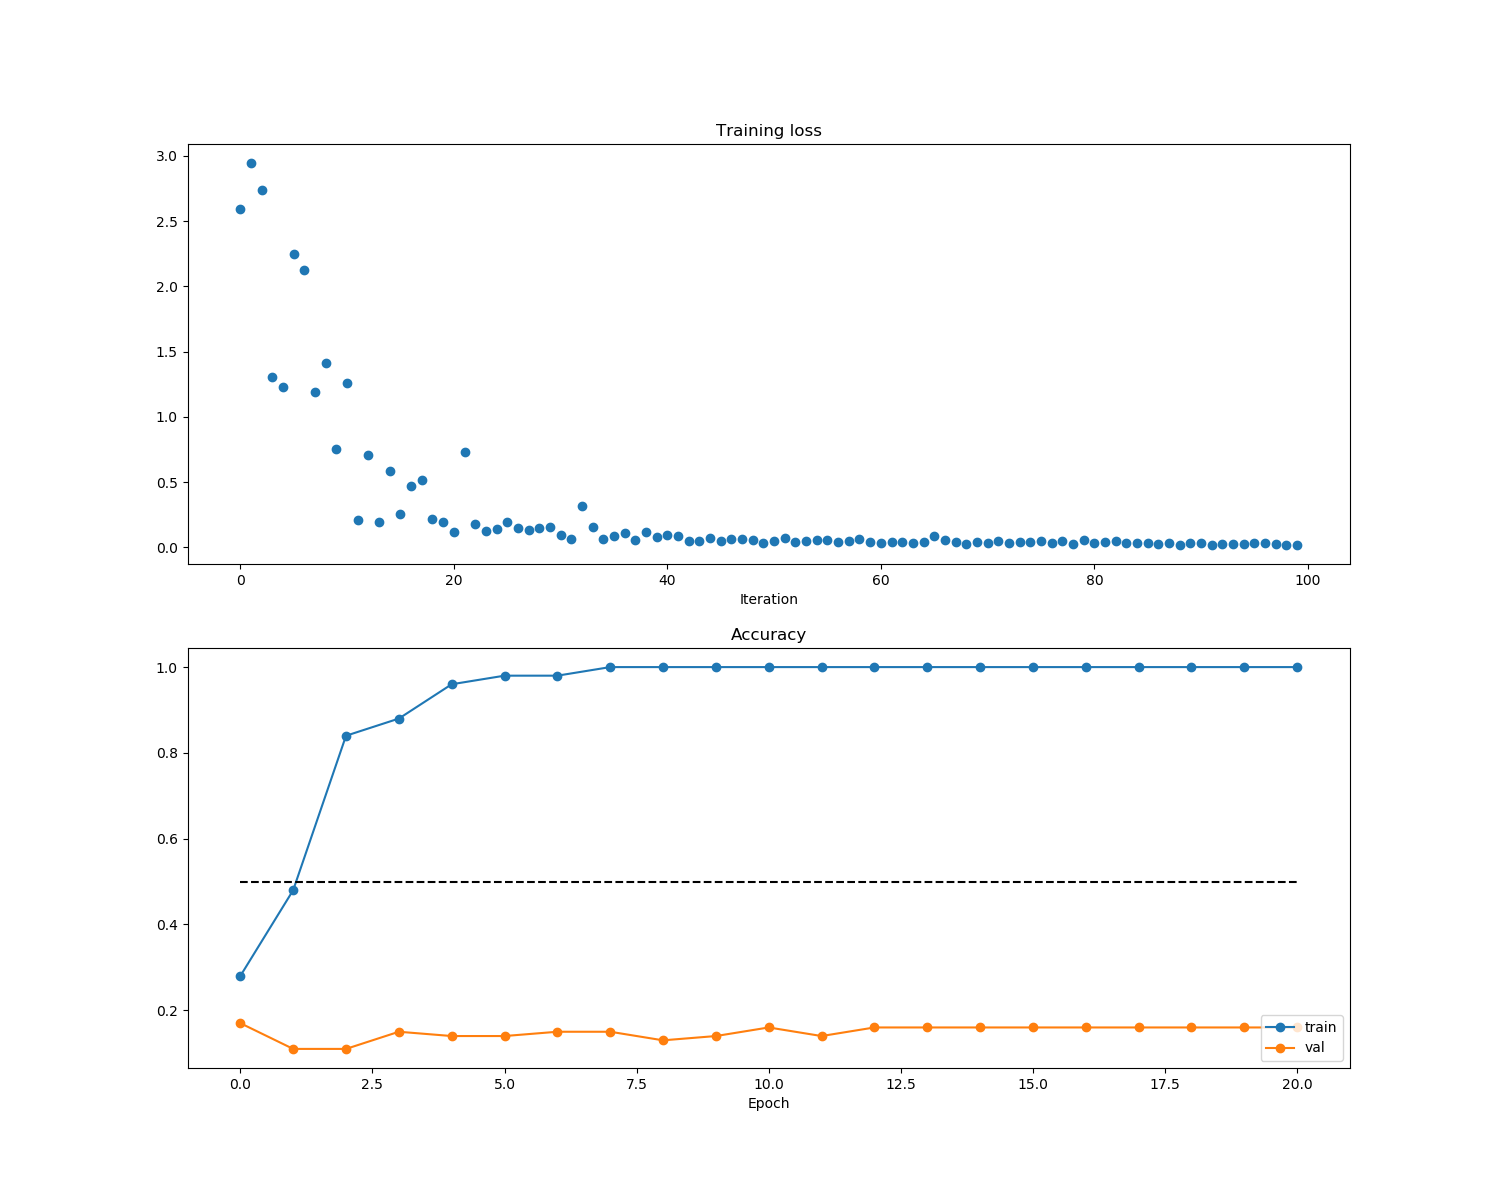
\includegraphics[width = 0.8\hsize]{./figures/overfit.png} % this includes the figure and specifies that it should span 0.7 times the horizontal size of the page
\caption{Network overfitting a subset of CIFAR10 dataset} % caption of the figure
% with a $stepsize$ $0.06$ and starting point $[1, -1]^T$
\label{fig:overfit} % a label. When we refer to this label from the text, the figure number is included automatically
\end{figure}

\begin{figure}[H]
\centering % this centers the figure
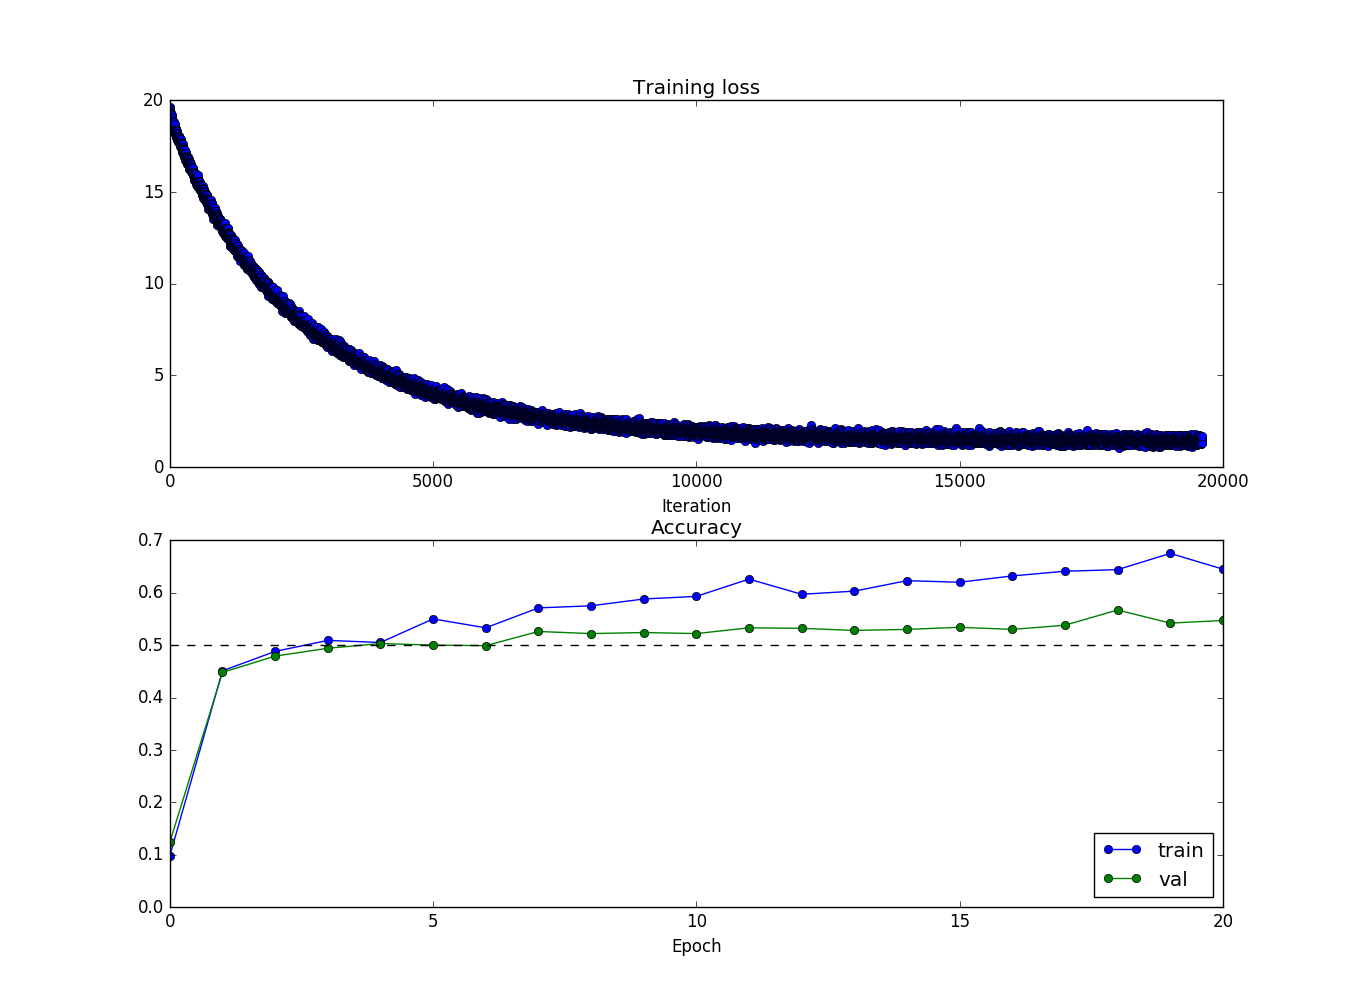
\includegraphics[width = 0.8\hsize]{./figures/cifar_2layer.png} % this includes the figure and specifies that it should span 0.7 times the horizontal size of the page
\caption{Network achieving $>50\%$ validation accuracy in CIFAR10 dataset} % caption of the figure
% with a $stepsize$ $0.06$ and starting point $[1, -1]^T$
\label{fig:cifar_2layer} % a label. When we refer to this label from the text, the figure number is included automatically
\end{figure}

\subsection{Question 5}
Select a reasonable network architecture as starting point and explain the motivation to choose so. 
Define a stopping criterion and a momentum and learning rate update schedule. 
You needto apply the stopping criterion to the solver (src/utils/solver.py).
Optimise the learning rate (disable regularisation). 
Explain how you found a good initial valuefor learning rate. 
Include the plot for training and validation loss and report training and vali-dation classification error.
Use dropout and report if there is any improvement in the validation performance.
You have implemented dropout and L2 as ways of regularisation. 
Use L2 and compare the performance with dropout.
Optimise the topology of the network, i.e. the number of hidden layers and the number of neurons in each hidden layer.

\subsection{Question 6}
For this task we used Tensorflow and built three different models. The first model we built is ha sthe following layers:

\begin{itemize}
\item input layer of dimensions Nx48x48x1 (batch size x image width x image height x number of channels)
\item convolutional layer 1, 16x5x5x1 filters (number of filters x kernel width x kernel height x number of channels) at stride 1 and 2 zero padding at all dimensions, followed by ReLu activation. The 5x5 filters were chosen as a commonly used filter type and the stride and padding were selected so that the convolution layer does not modify the size of the features
\item max pool layer of size 2x2 (width x height) at stride 2 that performs dimensionality reduction. After this step the each feature's dimensions are halved leading to a tensor of dimensions Nx24x24x16 (batch size x image width x image height x number of features)
\item convolutional layer 2, 32x5x5x16 filters (number of filters x kernel width x kernel height x number of channels) at stride 1 and 2 zero padding at all dimensions, followed by ReLu activation. The 5x5 filters were chosen as a commonly used filter type and the stride and padding were selected so that the convolution layer does not modify the size of the features
\item max pool layer of size 2x2 (width x height) at stride 2 that performs dimensionality reduction. After this step the each feature's dimensions are halved leading to a tensor of dimensions Nx12x12x32 (batch size x image width x image height x number of features). This  layer is reshaped to a vector of dimension 4608 and dropout is applied
\item fully connected layer with 1024 nodes and dropout
\item output layer of dimension 7 as this is the number of classes we want to predict
\end{itemize}

The other two networks we used are variants of ResNet presnted in [1], [2], specifically the 50-layer and the 101-layer bottleneck networks. Residual networks are one of the most significant advances in terms of convolutional neural network architecture over the last decade. They use what the authors call skip connections between layers that pass identity mappings between the layers they connect. This is shown in Fig.\ref{fig:skip_connections} below. As a result the convolutional layers between skip connections have to model the residual function which is an easier task for the model. This architecture option results in more efficient backpropagation and the capacity to train far deeper models that was though achievable before.   

\begin{figure}[H]
\centering % this centers the figure
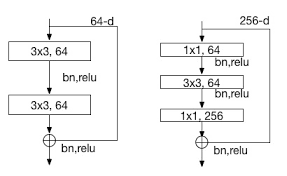
\includegraphics[width = 0.6\hsize]{./figures/skip_connections.png} % this includes the figure and specifies that it should span 0.7 times the horizontal size of the page
\caption{Residual networks building blocks. taken from [1]} % caption of the figure
% with a $stepsize$ $0.06$ and starting point $[1, -1]^T$
\label{fig:skip_connections} % a label. When we refer to this label from the text, the figure number is included automatically
\end{figure}

\newpage
\section{A1}
We could not claim one to be a better algorithm than the other in general for the following reasons stemming from the fact that the two methods are very different qualitatively:
\begin{itemize}
\item neural networks can be seen as black box function approximators while trees are highly interpretable. In cases where interpretability is crucial we could not use neural networks
\item fitting and doing inference with the two models scales differently depending on the software and hardware architecture used. The computing architecture of today might allow one model to be run more efficiently and outperform the other but that will not necessarily hold for tommorow's architectures
\end{itemize}
Finally, the no free lunch theorem of [3] states that no apriori distinctions can be made between any two learning algorithms. that is to say that while the inductive principle used by one model might allow it to overperform another at a given problem, when examined under the scope of all possible problems, any two learning algorithms are equivalent.


\section{A2}

For the classifcation trees, we will need to retrain the whole model as the addition of one class, because the space previously occupied by some classes wil need to be assigned to the new class.\\

For the case of neural networks a step we would definitely need to take is to add another node at the output layer of th enetwork allowing the classification of $n+1$ classes where the previous network was capable of classifying $n$ classes. We will need to initialize the wieghts and bias connecting the new node with the last layer and we will need to train at least the last layer of the network. most possibly we will need to retrain the other layers but the previously trained network will provide a good initialization, so we will not need to start from scratch.


\newpage
\section{Instructions for executing}
All code was written in Python3. All scripts were tested and run in the DOC Lab environment. To run the submitted scripts open a terminal window in the project directory and follow the instructions below.\\

\newpage
\section{References}

\begin{verbatim}
[1] Kaiming He, Xiangyu Zhang, Shaoqing Ren, Jian Sun
    Deep Residual Learning for Image Recognition. arXiv:1512.03385

[2] Kaiming He, Xiangyu Zhang, Shaoqing Ren, Jian Sun
    Identity Mappings in Deep Residual Networks. arXiv: 1603.05027
    
[3] Wolpert, David (1996), "The Lack of A Priori Distinctions between Learning Algorithms", Neural Computation, pp. 1341-1390
\end{verbatim}


\end{document}
%%% Local Variables: 
%%% mode: latex
%%% TeX-master: t
%%% End: 
